% !TEX root = main.tex

%%%%%%%%%%%%%%%%%%%%%%%%%%%%%%%%%%%%%%%%%%%%%%%%%%%%%%%%%%%%%%%%%%%%%%%%%%%%%%%%%%%%%%%%%%%%%%%%%%%%%
%
%   Version     : 4.0
%
%   Filename    : main.tex
%
%   Description : This is the main file for the LaTeX thesis proposal document template.
%                 The template is intended for use by students under the Department of Software Technology. 
%
%                It is assumed that you can learn how to use LaTeX on your own.
%                Please check/read the following online LaTeX book:
%
%                                 http://en.wikibooks.org/wiki/LaTeX
%     
%   Author      : Florante R. Salvador
%
%   Contributors: 1.  Karlo Campos (former faculty member)
%                 2.  Briane Paul V. Samson 
%   
%   Notes       : Please email the DST Thesis Coordinator, Mr. Edward Tighe (edward.tighe@dlsu.edu.ph), for feedback and suggestions
%
%   Reference:
%
%
%   History/Updates:
%      March 12, 2009:
%           -- created version 1.0 for release to CSC701M (Methods of Research) students
%      May 30, 2009   
%           -- updated Title page and Abstract for undergrad ST students
%      Feb 27, 2015 (version 2)
%           -- changed class to report, created a figures folder, 
%              removed unnecessary packages, added new comments  based on Ethel Ong's slides
%      Feb 24, 2018 (version 3)
%           -- Reorganized the chapters, i.e., Chapter 3 is now Theoretical Framework 
%              and Chapter 4 is now Research Methodology.
%           -- Included the Research Ethics documents as Appendix A.
%      June 15, 2022 (version 4)
%           -- Updated the title page
%           -- Revised text for figures and references
%
%%%%%%%%%%%%%%%%%%%%%%%%%%%%%%%%%%%%%%%%%%%%%%%%%%%%%%%%%%%%%%%%%%%%%%%%%%%%%%%%%%%%%%%%%%%%%%%%%%%%%%

%%%%%%%%%%%%%%%%%%%%%%%%%%%%%%%%%%%%%%%%%%%%%%%%%%%%%%%%%%%%%%%%%%%%%%%%%%%%%%%%%%%%%%%%%%%%%%%%%%%%%%%%%%%%%%%%%%%%%%%
%
%  Filename   : preamble.tex
%
%  Description: Preamble file to :
%               a. specify related packages
%               b. set margins, commands, etc.
%
%  Note       : Edit the margin settings for your own printer
%                  You may add your own commands, environments (it is assumed that you know what you're doing.)
%
%%%%%%%%%%%%%%%%%%%%%%%%%%%%%%%%%%%%%%%%%%%%%%%%%%%%%%%%%%%%%%%%%%%%%%%%%%%%%%%%%%%%%%%%%%%%%%%%%%%%%%%%%%%%%%%%%%%%%%%

%\documentclass[12pt,titlepage,onepage, letterpaper]{article}


\documentclass[12pt,titlepage,onepage,letterpaper]{report}


%
%-- specify related packages
%

%
% \usepackage[utf8x]{inputenc}
%

\usepackage{pdfpages}

\usepackage{apacite}           %-- APA style citation 
                               %-- refer to http://www.ctan.org/tex-archive/biblio/bibtex/contrib/apacite/

%
%  \usepackage{ucs}
%


\usepackage{amsmath}           %-- American Math Society packages
\usepackage{amsfonts}
\usepackage{amssymb}
\usepackage{booktabs}

\usepackage{graphicx}          %-- graphicx package needed for including figures in JPG or PNG format
 
%
%\usepackage{graphics}          %-- graphics related package (this was commented out) use when image is in EPS format
%

\usepackage{verbatim}          %-- this package allows you to have multiple lines of comments by
                               %-- example:
                               %   \begin{comment}
                               %        ...your text here...
                               %   \end{comment}  

\usepackage{color}             %-- allows use of color with text
                               %-- example:  \textcolor{red}{This is the colored text in red.}

\usepackage{url}  %-- allows use of URLs example: \url{https:\ccs1.dlsu.edu.ph}


%
%-- set margins,  you may need to edit this for your own printer
%
\topmargin 0.0in
\oddsidemargin 0.0in
\evensidemargin 0.0in

\voffset 0.0in
\hoffset 0.5625in

\textwidth 5.75in
\textheight 8.5in


\parskip 1em
\parindent 0.25in

\bibliographystyle{apacite}            %-- use APA citation scheme

\hyphenation{ana-lysis know-ledge}     %-- LaTeX may not hyphenate correctly some words you use in your document
                                       %-- use \hyphenation to instruct LaTeX how to do it correctly, example above

\newcommand{\degree}{^{\circ}}         %-- use \newcommand to create your own "commands"
                                       %-- \newcommand works like the #define you learned in your COMPRO1 class

\newcommand{\etal}{et al.}


%\newcommand{\sinag}{\emph{Sinag}}
%\newcommand{\sinagtwo}{\emph{Sinag2}}

\newcommand{\figref}[1]{Figure \ref{#1}}
\newcommand{\appref}[1]{Appendix \ref{#1}}

%-- \newcommand{\Section}[1]{\section{#1}\setcounter{figure}{0}\setcounter{table}{0}}

%\newcommand{\shade}{\multicolumn{1}{|>{\columncolor[gray]{0.25}}c|}{}}
%\newcommand{\tableheader}[1]{\rowcolor{black}\color{white}{#1}}
%\newcommand{\cell}[2]{\multicolumn{1}{#1}{#2}}
%\newcommand{\definition}[2]{\textbf{\textit{#1}} --- #2}
%\newcommand{\itembit}[1]{\item \textbf{\textit{#1}}}
%\newcommand{\sgdef}[2]{\parbox[t][][t]{1.75in}{\textbf{#1}} \> \parbox[t][][t]{4.0in}{#2}\\\\}

%\newenvironment{sinagglossary}{\begin{flushleft}
%\begin{tabbing}
%\hspace{1.75in}\=\\}{\end{tabbing}\end{flushleft}}

\newcommand{\thestitle}[1]{{\Large \textsc{#1}}}


%---
%  \renewcommand{\thefigure}{\thesection.\arabic{figure}}
%  \renewcommand{\thetable}{\thesection.\arabic{table}}
%  \renewcommand{\contentsname}{Table of Contents}

                %-- includes LaTeX source file for the preamble 
                                  %-- include packages, sets the margin sequence, and many more... 
                                  %-- your job: check if the settings are suitable for your own printer

\graphicspath{{figures/}}  %-- figures is the name of the folder containing images JPG or PN

\begin{document}

%%%%%%%%%%%%%%%%%%%%%%%%%%%%%%%%%%%%%%%%%%%%%%%%%%%%%%%%%%%%%%%%%%%%%%%%%%%%%%%%%%%%%%%%%%%%%%%%%%%%%%
%
%   Filename    : title_page.tex 
%
%   Description : This file will contain your Title Page.
%                 
%%%%%%%%%%%%%%%%%%%%%%%%%%%%%%%%%%%%%%%%%%%%%%%%%%%%%%%%%%%%%%%%%%%%%%%%%%%%%%%%%%%%%%%%%%%%%%%%%%%%%%

\begin{titlepage}
\centering


%-- **EDIT** the following line to indicate your thesis title. Try to keep it within 20 words for brevity, and focus on highlighting the intended contribution of your work.
\thestitle{A Study on the use of Augmented Reality on Bataan Death March For game based learning and affective learning}

\vspace{1.5cm}

A Thesis Proposal\\

\vspace{0.5cm}

presented to\\

\vspace{0.5cm}

the Department of Software Technology\\
College of Computer Studies\\
De La Salle University

\vspace{1cm}

In partial fulfillment\\
of the requirements for the degree of\\

\vspace{0.5cm}

%Master of Science in Computer Science
Bachelor of Science in Computer Science\\
Major in Software Technology
\vspace{1.75cm}
\\by\\


%% EDIT the following line to indicate the complete names of all your group members arranged in alphabetical order 
\vspace{1cm}

CUSTER, Mark John Tiamzon  \\
PARK, Sehyun \\
SILLONA, John Eugene Justiniano  \\
TUCO, Kevin Bryan Layugan  \\

\vspace{1.75cm}
%-- **EDIT** the following line to indicate your adviser's name 
Christian Terrence Esguerra \\
Adviser

\vspace{1.25cm}
\today
\end{titlepage}
              %-- includes LaTeX source file for the Title Page 
                                  %-- your job: **EDIT THIS FILE ** to indicate your own title, name, and thesis adviser's name


%%%%%%%%%%%%%%%%%%%%%%%%%%%%%%%%%%%%%%%%%%%%%%%%%%%%%%%%%%%%%%%%%%%%%%%%%%%%%%%%%%%%%%%%%%%%%%%%%%%%%%
%
%   Filename    : abstract.tex 
%
%   Description : This file will contain your abstract.
%                 
%%%%%%%%%%%%%%%%%%%%%%%%%%%%%%%%%%%%%%%%%%%%%%%%%%%%%%%%%%%%%%%%%%%%%%%%%%%%%%%%%%%%%%%%%%%%%%%%%%%%%%

\begin{abstract}
History class has always been a trouble for students due to its nature in memorization for an exam-based classroom settings and requires an ability to visualize the events through word and pictures. Game-based learning such as simulations has risen to be effective in getting the attention of the students due to their inherent appeal and similarity to games; from which students and teens alike play worldwide. There has been numerous studies on game-based learning to overcome this problem but there are limited studies on simulations and integrating augmented reality technology into classroom settings, with few studies found within the Philippines'. This study aims to close the gap by developing mobile-based AR simulation application, and provide insights into its applicability and effectiveness within the Philippines’ educational system, and additonally assess the effects of different AR components on student performance through an analysis of interactive elements, historical content representations, and immersive feature. 

\begin{flushleft}
\begin{tabular}{lp{4.25in}}
\hspace{-0.5em}\textbf{Keywords:}\hspace{0.25em} & Game-based learning, Augmented  reality, Education
\end{tabular}
\end{flushleft}
\end{abstract}
                %-- this is the Abstract page
                                  %-- your job: **EDIT THIS FILE** to indicate your own abstract

\pagenumbering{roman}             %-- this will number pages as i, ii, iii, etc...
\setcounter{page}{2}

\tableofcontents                  %-- this command is used to generate the Table of Contents


%\newpage
%\listoffigures                    %-- this command is used to generate List of Figures

%\newpage                       
%\listoftables                     %-- this command is used to generate List of Tables

\newpage

\pagenumbering{arabic}            %-- this will number pages as 1, 2, 3, etc...
\setcounter{page}{1}              


%%%%%%%%%%%%%%%%%%%%%%%%%%%%%%%%%%%%%%%%%%%%%%%%%%%%%%%%%%%%%%%%%%%%%%%%%%%%%%%%%%%%%%%%%%%%%%%%%%%%%%
%
%   Filename    : chapter_1.tex 
%
%   Description : This file will contain your Research Description.
%                 
%%%%%%%%%%%%%%%%%%%%%%%%%%%%%%%%%%%%%%%%%%%%%%%%%%%%%%%%%%%%%%%%%%%%%%%%%%%%%%%%%%%%%%%%%%%%%%%%%%%%%%

\chapter{Introduction}
\label{sec:intro}   
\section{Background of the Study}
\label{sec:overview}

History is normally taught with traditional methods such as lectures and discussions. As it requires high levels of understanding, the youth often avoids history. There are other methods that lecturers utilize in teaching history, such as creative means like audio-visual presentations, software, and interactive means. Video games, especially a simuations provide an excellent example of interactive and affective learning \cite{ARVRRome}. Not only is it popular among the new generation, but it grants freedom to choose however they may play the game and achieve different results based on their playstyle.
 
\subsection{Students' Hardship in Classes}
There are multiple factors which makes a student lose their interest and participation in a typical classroom settings. Some of the factors include easy or difficult materials, lack of interest in a subject, and a lecture-based environment \cite{medium:mosley}. Out of all the problems which causes the students to disconnect from the act of learning, test-driven classroom culture was one of the biggest factor which significantly impacts students' educational experience \cite{mora}. The student's negative view of the classroom primarily focused on multiple standardized test they needed to prepare, and how classes were centered around these tests rather than students.

The same study by \cite{mora} showed how students were less bored and engaged when the classes were integrated with more interactive and hands-on activities such as poster-making and science experiments, rather than typical lecture based classroom set ups. This behavior of the students opens up to the possibility of integrating augmented reality simulation based learning material to enhance the involvement of the students to the class and further enhance their performances by creating a student-centered environment.


\subsection{Utilization of Augmented Reality with Affective Learning}
Technological advancements are enhancing the education of students \cite{lamp2024}. Included in these advancements are virtual reality, mixed reality, and augmented reality. Most studies that are mentioned here have shown that using extended reality technologies have a positive impact with the way that students learn.

A study was conducted to investigate if augmented reality can promote learners' emotional and cognitive connection to a puzzle game that contains local cultural knowledge \cite{tsai2024}. The experimental group was given information using augmented presentations through a smartphone. On the other hand, the control group was provided with paper-based materials. The results show that combining augmented reality with the puzzle game have shown an increase in their understanding and their immersion with unique historical and geographical contexts. Additionally, it has also shown that the experimental groups have maintained their memory much longer.

To further support their correlation, a study by Lampropoulos et. al. has compiled 188 editorials and used bibliometric analysis and scientific mapping approach to create a general trend on extended reality technologies. The results show that there is a strong relationship between augmented reality and affective learning/computing. One particular example was implementing augmented reality with engineering education which has further increased the affective states of students, emotions, behaviors, preferences, and actions.


\section{Research Objectives}
The project aims to develop an augmented reality simulation application that includes affective learning to enhance the user's understanding of historical events, focusing on the Bataan Death March. The researchers aims to investigate and address the factors causing student's difficulties in history classes and develop strategies to enhance student's learning experience using augmented reality.

The specific objective of this project is directed into answering these following questions
\begin{enumerate}
    \item Can augmented reality technology be improved such that it would be utilized to create an immersive environment for the users?
    \item How can the integration of augmented reality simulations aid in teaching history through the use of affective learning?
    \item How do students assess the effectiveness of augmented reality simulations in improving their comprehension and engagement with historical events? 
\end{enumerate}

The expected outcome of this project is to develop a mobile-based augmented reality simulation application with Unity engine with Vuforia add-on, which the student's can utlize to experience the Bataan Death march with immersive atmosphere. The application will immerse the user in a first-person perspective of the victim of the Bataan Death March and guide them through the event. Dialogues describing the actual historical event will be incorporated into the simulation gameplay for user interaction, enhancing the application's historical value for education. The users are expected to learn and absorb the historical event of Bataan Death March through affective learning at the end of the simulation, leading to a deeper understanding of the event compared to traditional classroom settings.
 
\section{Scope and Limitations}
\subsection*{Scope}
This study will focus on implementing augmented reality into historical learning as well as identifying the possible frameworks, technologies, and practices in developing augmented reality software assisting in learning.
\

\subsection*{Limitation}
The proposed Augmented Reality Simulation will depict fictionalized events and scenarios of the Bataan Death March. It will observe multiple events that may or may not have happened based on recorded histories and captured footage. Thus, the proposed simulation will only be partially historically accurate and authentic.

\section{Significance of the Study}
This project will further allow augmented reality technology to be incorporated in the field of education and allow different teaching strategies to be developed for the students. There are multiple studies abroad with utilization of game-based learnings and their integration into a classroom settings \cite{watson2011}. Despite the growing interest and advancements in augmented reality applications for education globally, the related studies are scarcely found in the Philippines. This project aims to address this gap by developing a mobile-based AR simulation application, and provide insights into its applicability and effectiveness within the Philippines' educational system. This research will offer valuable data on how AR can be adapted to meet the Philippines' educational needs and challenges. Additonally, This project aims to assess the effects of different augmented reality components on student performance through an analysis of interactive elements, historical content representations, and immersive features. The goal is to determine which elements within the AR technology are most successful in enhancing student engagement,  comprehension, and retention of historical events at the end of the project.
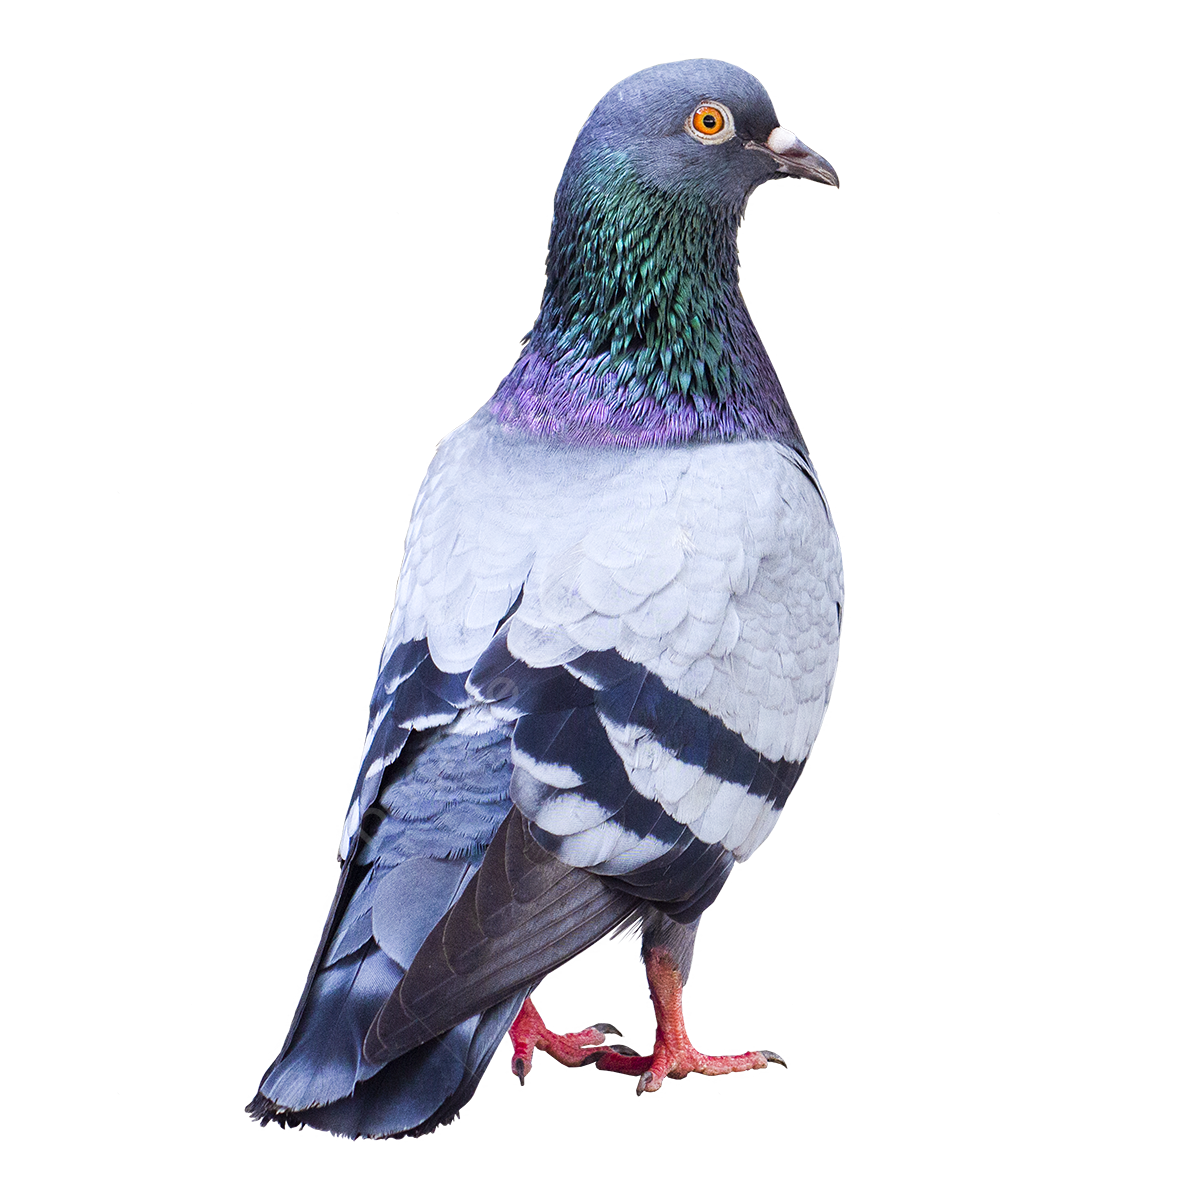
\includegraphics{sample.png}

               %-- includes LaTeX source file for Chapter 1: Research Description
                                  %-- your job: **EDIT THIS FILE** to indicate your own research description

%%%%%%%%%%%%%%%%%%%%%%%%%%%%%%%%%%%%%%%%%%%%%%%%%%%%%%%%%%%%%%%%%%%%%%%%%%%%%%%%%%%%%%%%%%%%%%%%%%%%%%
%
%   Filename    : chapter_2.tex 
%
%   Description : This file will contain your review of related works.
%                 
%%%%%%%%%%%%%%%%%%%%%%%%%%%%%%%%%%%%%%%%%%%%%%%%%%%%%%%%%%%%%%%%%%%%%%%%%%%%%%%%%%%%%%%%%%%%%%%%%%%%%%

\chapter{Related Works}
\label{sec:relatedworks}
\begin{comment}
%
% IPR acknowledgement: the contents within this comment are from Ethel Ong's slides on RRL.
%
Guide on Writing your Related Works chapter
 
1. Identify the keywords with respect to your research
      One keyword = One document section
                Examples: 2.1 Story Generation Systems
			 2.2 Knowledge Representation

2.  Find references using these keywords

3.  For each of the references that you find,
        Check: Is it relevant to your research?
        Use their references to find more relevant works.

4. Identify a set of criteria for comparison.
       It will serve as a guide to help you focus on what to look for

5. Write a summary focusing on -
       What: A short description of the work
       How: A summary of the approach it utilized
       Findings: If applicable, provide the results
        Why: Relevance to your work

6. At the end of each section,  show a Table of Comparison of the related works 
   and your proposed project/system

\end{comment}

\section{Difficulty in Classes}
There are multiple factors which affects students' hardship in classes \cite{cmu}.
\begin{enumerate}
    \item Students may not see value in their curriculum
    \item Students does not believe their work will increase their performance
    \item Demotivated by the results and reward
    \item Restricted classroom environment
    \item Physical, mental, or other personal problems
\end{enumerate}
The examples above doesn't describe all but some of the significant factors which students are mostly affected with. There were several attempts in previous studies where some of these factors were negated with an integration of game-based learning in classrooms. \cite{watson2011} developed and introduced a video game to the classroom to teach students about World War II. Their study was able to turn static classroom environment into more friendly student-centered class and amplify the students' participation with the learning module. \cite{Hara} evaluated an effectiveness of an augmented reality application called \textit{Historic Augmented Reality Application} to increase an involvement of students by integrating a software where students can be interacted with the learning materials within the classroom environment. Their study was able to prove the improvement of students' attention span within the class with the usage of AR application and occupy them with discussions and class participation. These studies from the past have proven the game-based learning's positive effects, as well as its side effects thoroughly. It is essential to analyze and understand why game-based learning enhances the performance of some students while proving less effective for others. Understanding these factor is crucial for pinpointing what specific conditions or variables contribute to the efficacy or ineffectiveness to this approach.

\begin{comment}
    

\section{Clickers in Classroom}
There has been numerous attempt to gain back students' attention in class through the usage of an external tools. Clickers, one of the tools which was used by the teachers in the classroom settings introduced inter-activeness between the student and a teacher by promoting a classroom response systems. Clickers utilizes a remote control which a students can use to take attendance, answer a multiple choice questions, or to kick start a discussion within the class \cite{tophat:persaud}. A data in the study by \cite{clickers2010} suggests that most of the students attention alternates between an engaged and non-engaged state in a short cycle of 10-20 minutes. Within the span, the students are easily distracted by other dues such as doing homework for other class or checking their texts and social networks. The study also suggests that the usage of external tools such as Clickers to demonstrate and ask a question to the class significantly increased the attention of the students compared to the lecture-based learning materials and reduced distracted behaviors from the students. 

Unfortunately, there is always a challenge when introducing an external tools to the classroom. Firstly, the institution must have sufficient funds to approve the cost that will be associated with implementation. This involves not just a hardware but also setting up sufficient environment, such as a supplying a consistent WI-FI bandwidth across the entire classrooms. They must also invest in time in educating teachers to efficiently use certain tool in class. Additionally, an external tool - specifically Clickers has the potential to be misused by the students. A student can simply fake their friends' attendance or answer a question for them which will affect their understanding of a module, and cause a long-term effect in their studies \cite{tophat:persaud}. 

While introduction of an external tools to enhance the students' attention and create a more student-centered environment seems to be effective, it must always be approached with caution to prevent an exploitation of a tool by students. It is the responsibility of both the teacher and the creator of the tool to understand the students' frustration in class and address them accordingly. 
\end{comment}

\section{Game Based Learning}
Game based learning is a learning technique which utilizes a game either digitally or non-digitally to increase a performance of a student by enhancing critical thinking and problem solving skills and creating student-centered environment in classes \cite{tophat:tamosevicius}. Some of the known example of the game based learning includes Menti, Kahoot, Handmade Board games, and real-life games which involves physical participation of the student.

Data from several case studies involving the integration of game-based learning into classrooms shows its effectiveness in improving student performance. A study from \cite{gameOn} showed increase in students' preference and engagement from gamified lectures, and their ability to interact and share ideas reported to be more effective and amplified. Another study from \cite{watson2011} involved \textit{Making History} - a video game designed with an educational purpose to teach students the history of World War II. This case study showed how the integration of game-based learning into a standard American classroom was able to convert the restricted teacher-centered classroom where students were mostly passive into a more student-centered environment which made students more engaged and less hesitant to share their ideas to the class.  

While game-based learning does provide positive effects toward students, there are side effects which may occur if not integrated properly to the class. In recent years, there has been an increase in phenomena of \textit{Gaming the System}, where learners attempt to exploit the education system to achieve a high performance rather than attempting to absorb the lessons \cite{baker2008}. It is important to understand why students choose to game the system to create a educational that students do not attempt to exploit it.

According to \cite{malone1980fun} in his study on what makes things fun to learn, there are certain criteria which needs to be considered to create an effective game for education. 1. The game must have clear goal and must be compelling, 2. The player must know if they are getting closer to the goal, 3. Game should provide varying difficulty for the varying skill levels of the players. Another insight from \cite{mozelius2017} in the perspective of the games that will be used for education must be 1. Not to costly, and must be easy to install, 2. The game should be playable under 40 minutes to be used in a classroom settings, 3. If not, the game is better to be used as a homework instead. These criteria from the previous studies must be carefully observed and integrated into the project accordingly to avoid exploits from the students.  

\section{Affective Learning and World War II History}
According to Mahadeo and Nepal (2023), a teaching method that recognizes the vitality of emotions in learning improves students' experience, creating a positive and effective outcome. Affective Learning, as defined, is the process of learning skills and attitudes through emotional engagement. It enhances curiosity and enthusiasm in learning outcomes that foster a deeper understanding of the context with meaningful retention of information. It is an approach that tailors to cognitive and emotional dependency to promote holistic and impactful learning experiences. Nurturing positive emotional experiences can improve student engagement, critical thinking, and academic performance by creating a transformative learning experience that allows personal and educational growth.

The strategy of using Affective Learning in teaching World War II History can affect how the students can see the gravity of the effects of war on the country and the people without having to experience it and by only seeing it through the lens of those who lived it. A study by Kim et al. (2019) showed the hardships of comfort women during World War II. The Japanese Military during World War II created comfort stations that used women as tools for relief, stripping the dignity and freedom of the comfort women. The study used male and female students of diverse ethnicities to interview comfort women survivors who narrated their experiences. One of the students said that he learned the facts about comfort women in class, but hearing the reality from the person who survived made the history "more real." According to Waters and Russell III (2012), the violation of human rights in the context of history should be taught in social studies classrooms to help students become better citizens. Discussing and exploring the issues of human rights violations in the context of World War II history helps students conceptualize and identify current human rights violations while stating that mere recognition of injustices is not enough to pursue actions.

\section{Historic Augmented Reality Application (HARA)}
There has been several studies on applying augmented reality (AR) technology into education to amplify the learning of the students and create an immersive environment for them \cite{ARVRRome}. Although there are numerous studies from various parts of the world, there are few papers discussing the application of AR technology in school settings in the Philippines. 

Historic Augmented Reality Application (HARA) is an application developed in the Philippines which aims to teach students the Philippines-American colonization period through immersive story telling \cite{Hara}. The application aimed to teach students the three distinct event during the American colonization, namely the battle of manila bay, mock battle of manila, and the first shot in Philippines-American war. 

HARA is a mobile-based application integrated with AR technology, and the decision was made to develop it using the Unity and Vuforia engine. This choice was influenced by Unity's capability to publish across over 25 platforms compared to other suitable mobile development platforms such as Android Studio, and technical aspect of how Vuforia engine is easily co operable with Unity engine was another factor in the decision making. The HARA relies on image recognition of the predefined set images through the cameras of the mobile phones, after which the application overlays a 3D animated scene displaying the event shown in the images. The development of the HARA lasted from May to October of year 2018, with first four months spent on development and beta release of the application, and final two for user evaluation and modification. 

HARA was the first application in the Philippines which utilizes augmented reality with 3D animated scenes to be used to teach history in a classroom setting. As a pioneering application in the field, to ensure the standard in the field of human-computer interaction field, the application usability was surveyed with a questionnaire based from the works of Guimarães and Martins which is used to evaluate AR application in terms of variables such as effectiveness, efficiency, and such by the co-designers of the application. The application received 82 percentage markings on its effectiveness, but received poor markings on satisfaction - 51, and efficiency - 43 from the co-designers due to factors such as slow animation and loading time. While the designers weren't fully satisfied with the application, the overall qualitative feedback from the users were positive. The application received a high overall markings of 4.2 out of 5, and got positive reviews from both students and teachers. Overall, the HARA shows how the AR technology is a promising tool in a field of education to effectively create immersive environment for the students.

\section{EON-XR: The Urban Planning of Rome}
With the growth of popularity of video games worldwide and the advancement in the field of Augmented and Virtual reality \cite{enterpriseappstoday2023}, Augmented Reality (AR) is no longer a technology that is foreign towards the young audiences such as high school and college students around the world. With student's apparent lack of motivation to study \cite{medium:mosley} and their hardship in classes, there has been numerous case studies on integrating gamification into education to boost the student's performance in class \cite{watson2011}. 

The study on \textit{EON-XR}, stands out among similar works as it is a simulation video game embedded with both Augmented and Virtual reality technology and was developed to be used for educational purposes \cite{ARVRRome}. The application was developed for mobile settings using Unity with Vuforia engine plug-ins for AR. The models of the buildings and characters were made with a 3DS Max modeling tool, maximizing the details of each assets for greater user immersion. 

The students were allowed to utilize the AR portion of the application to observe the visualization of the city elements with an optional description on the side to further enhance the explanation. This activity was told to increase the educational value of the game, and is to amplify the immersion of the era for the students. Aside from its AR feature, the EON-XR application also provides the user with a virtual reality (VR) simulation to allow them to walk around the cities of ancient Rome and visit notable landmarks such as The Colosseum on foot. The user can roam around a pre-designed city or build a city on their own to create an immersive simulation to their liking. To increase the historical potential of the game, the developers added a scroll with information of notable buildings inside them which the users can read in first person upon entering the buildings. \textit{EON-XR} shows a strong evidence of AR and VR being utilized to create immersive environment for the users, and create suitable environment around them to absorb the information efficiently.


\section{A Deep Dive into Immersive Technology}
Immersive technology, which includes AR and VR, have an increased in scholarly attention through the years. With that attention, only a few studies have been done to discuss the current state of this kind of research. A literature review was done from 54 rigorously selected articles and their findings were summarized into one study; all to show the current state of immersive technology, and to give light on gaps on research \cite{suh2018}.

The study summarized and combined results and data from the set of studied ariticles into multiple tables and figures that show aspects of both VR and AR \cite{suh2018}. The literature review summarized that immersive technology is good at increasing learning effectiveness and engagement while also improving attitudes at said learning materials; the study also discussed that, to increase immersion and effectiveness, it is better to have interactive elements, even better they are collaborative in nature \cite{suh2018}.

The literature review delved deep into both AR and VR technology and points out key concepts that are important in the application of those technology. The study's findings will definately help in guiding the researchers in the creation of the simulation and to create an even more immersive and effective AR experience. Lastly, the study created a framework from which our project can be built upon as seen from the figure below \cite{suh2018}.

\begin{figure}[h]
    \centering
    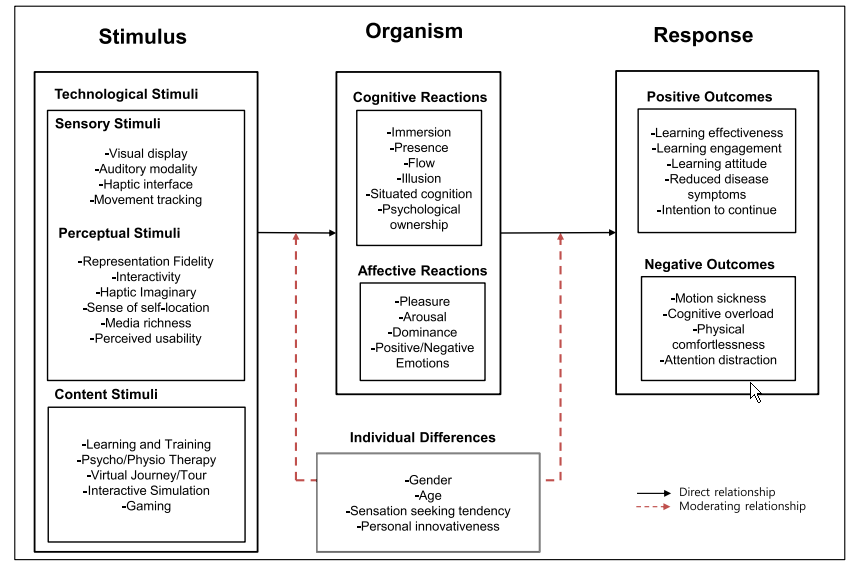
\includegraphics[width=0.8\textwidth]{figures/ImmersiveFramework.png}
    \caption{Immersive Technology Framework}
\end{figure}















               %-- includes LaTeX source file for Chapter 2: Review of Related Literature
                                  %-- your job: **EDIT THIS FILE** to indicate your review of related literature 

%%%%%%%%%%%%%%%%%%%%%%%%%%%%%%%%%%%%%%%%%%%%%%%%%%%%%%%%%%%%%%%%%%%%%%%%%%%%%%%%%%%%%%%%%%%%%%%%%%%%%%%
%
%   Filename    : chapter_3.tex 
%
%   Description : This file will contain your Theoretical Framework.
%                 
%%%%%%%%%%%%%%%%%%%%%%%%%%%%%%%%%%%%%%%%%%%%%%%%%%%%%%%%%%%%%%%%%%%%%%%%%%%%%%%%%%%%%%%%%%%%%%%%%%%%%%

\chapter{Theoretical Framework}
\label{sec:theoframework}
Please refer to the following resources regarding Theoretical Framework: 

\begin{itemize}

\item \url{https://link.springer.com/chapter/10.1007/978-1-4419-1454-5_12}
\item \url{https://link.springer.com/article/10.1007/s10972-015-9443-2}



\end{itemize}


               %-- includes LaTeX source file for Chapter 3: Theoretical Framework
                                  %-- your job: **EDIT THIS FILE** to indicate your research methodology

%\chapter{Methodology}
\label{sec:methodology}

This chapter enumerates and discusses the specific steps and activities that will be performed by the proponent to accomplish the objectives of the research. The discussion covers the activities from pre-proposal to Final Thesis Writing. 

Ethical issues surrounding the research and the steps to be taken by the research team to adhere to ethical guidelines and principles should be included when discussing each of the activities.

Research activities include inquiry, survey, research, brainstorming, canvassing, consultation, review, interview, observe, experiment, design, test, document, and other similar tasks. The following sections present an example set of activities and methods for conducting computing research. \textbf{\textcolor{red}{However, note that your group's actual research activities and methods will be different depending on your intended research contributions. You should consult closely with your thesis adviser for proper guidance. The following sections need not appear in your actual thesis proposal.}}

\section{Data Collection}

This section, also called "Data Gathering", focus on activities that will enable the researchers to understand their users and their context better, or to analyze the operating environment where the proposed software may be deployed. The types of activities would include interviews, observations, surveys, focus group discussions, and review of secondary data (reports, videos, manuals) to enable the researchers to identify user requirements; learn the existing processes, strategies, rules and guidelines; and/or build the datasets and knowledge resources needed in the study.

Ethical issues surrounding the collection of data from human participants, and from internet or 3rd party sources should be indicated. The steps to be taken by the proponents to ensure that ethical guidelines are followed should also be explained.

\section{Software Design and Implementation}

This section covers the design of data structures, knowledge bases, user interface, and algorithms. It includes implementation and related activities - tool selection, unit testing, integration testing, and function testing - that were covered in the course "Software Engineering".

Your Adviser may ask you to separate the Design and the Implementation sections as needed. 

You may also indicate a specific software development lifecycle model that you plan to adopt in developing your software, such as the Agile methodology.

For machine learning types of research, this section may be replaced with "Model Training".

\section{Validation}

This section contains the different types of validation activities that you will conduct to evaluate the performance of your model or algorithm or software. It may include user perception studies, end user acceptance testing, usability test, and model validation.

Ethical issues surrounding the collection of data from human participants should be indicated. The steps to be taken by the proponents to ensure that ethical guidelines are followed should also be explained.

This section should include a discussion of the following if working with human participants:
\begin{itemize}
    \item Participant Selection. Who are your target participants? How will they be selected? What data will be collected?
    \item Orientation. How will ethics be observed? What documents, e.g., validation protocol, will be shared with participants to orient them regarding the research and the validation procedure? Will there be an Informed Consent and Informed Assent? Are they found in the Appendix? Will there be any pre-tests or interviews to be administered prior to the actual experiment?
    \item Experiment Proper (aka Procedure). How long is the experiment or how long should the user use your software? Is it one-on-one, or one-to-many? What will you do while the experiment is ongoing - observe the participants using a checklist, guide the participants, record the interaction/usage?
    \item Debriefing. After the experiment, will you administer any post-tests or debriefing to solicit feedback from your participants? What are these?
\end{itemize}

\subsection{Calendar of Activities}

For the proposal, a Gantt chart showing the schedule of the activities should be added. You can create a table like below, or create a figure. For example:

Table \ref{tab:timetableactivities} shows a Gantt chart of the activities.  Each bullet represents approximately one week worth of activity.

\begin{table}[]
    \centering
    \begin{tabular}{l|c|c|c|c|c|c|c|c|c}
         \toprule
         & \multicolumn{6}{c|}{2021} & \multicolumn{3}{c}{2022} \\
         \textbf{Activity} & \textbf{Apr} & \textbf{May} & \textbf{Jun} & \textbf{Jul} & \textbf{Aug} & \textbf{Sep} & \textbf{Jan} & \textbf{Feb} & \textbf{Mar} \\
         \midrule
         Data Collection & **** & **** & & & & & & & \\
         \midrule
         Software Design & & **** & **** & **** & **** & **** & & & \\
         \midrule
         Validation & & & & & & **** & **** & **** & \\
         \bottomrule
    \end{tabular}
    \caption{Gantt Chart of Activities}
    \label{tab:timetableactivities}
\end{table}               %-- includes LaTeX source file for Chapter 4: Research Methodology
                                  %-- your job: **EDIT THIS FILE** to indicate your research methodology

% \appendix                         %-- used to specify appendices
% %%%%%%%%%%%%%%%%%%%%%%%%%%%%%%%%%%%%%%%%%%%%%%%%%%%%%%%%%%%%%%%%%%%%%%%%%%%%%%%%%%%%%%%%%%%%%%%%%%%%%%
%
%   Filename    : appendix_A.tex 
%
%   Description : This file is for including the Research Ethics Documents (delegated as Appendix A) 
%                 
%%%%%%%%%%%%%%%%%%%%%%%%%%%%%%%%%%%%%%%%%%%%%%%%%%%%%%%%%%%%%%%%%%%%%%%%%%%%%%%%%%%%%%%%%%%%%%%%%%%%%%

\chapter{Research Ethics Documents}
\label{sec:appendixa}


\begin{comment}

IMPORTANT -- READ THIS PART!!!

Please follow the instructions below on how to include the Research Ethics documents 
in your proposal document (typeset using LaTeX):

1. Open, and accomplish the contents of the THREE Word DOCX files included in the distribution

2. Once you're done filling in the necessary items, save the file in PDF format.  This is done by clicking on "File", 
    then "Save As" and then choose PDF (not DOCX default option) .  Do this for the three documents.

   The filenames are long, so I renamed the files with shorter names: 
       a . clearance.PDF  (original was GradSchool-revised ethics clearance form)
       b. general_checklist.PDF (original was General Research Ethics Checklist)
       c.  checklist-A PDF (original was [Specific Checklists] Checklist A - Human Participants]

\end{comment}


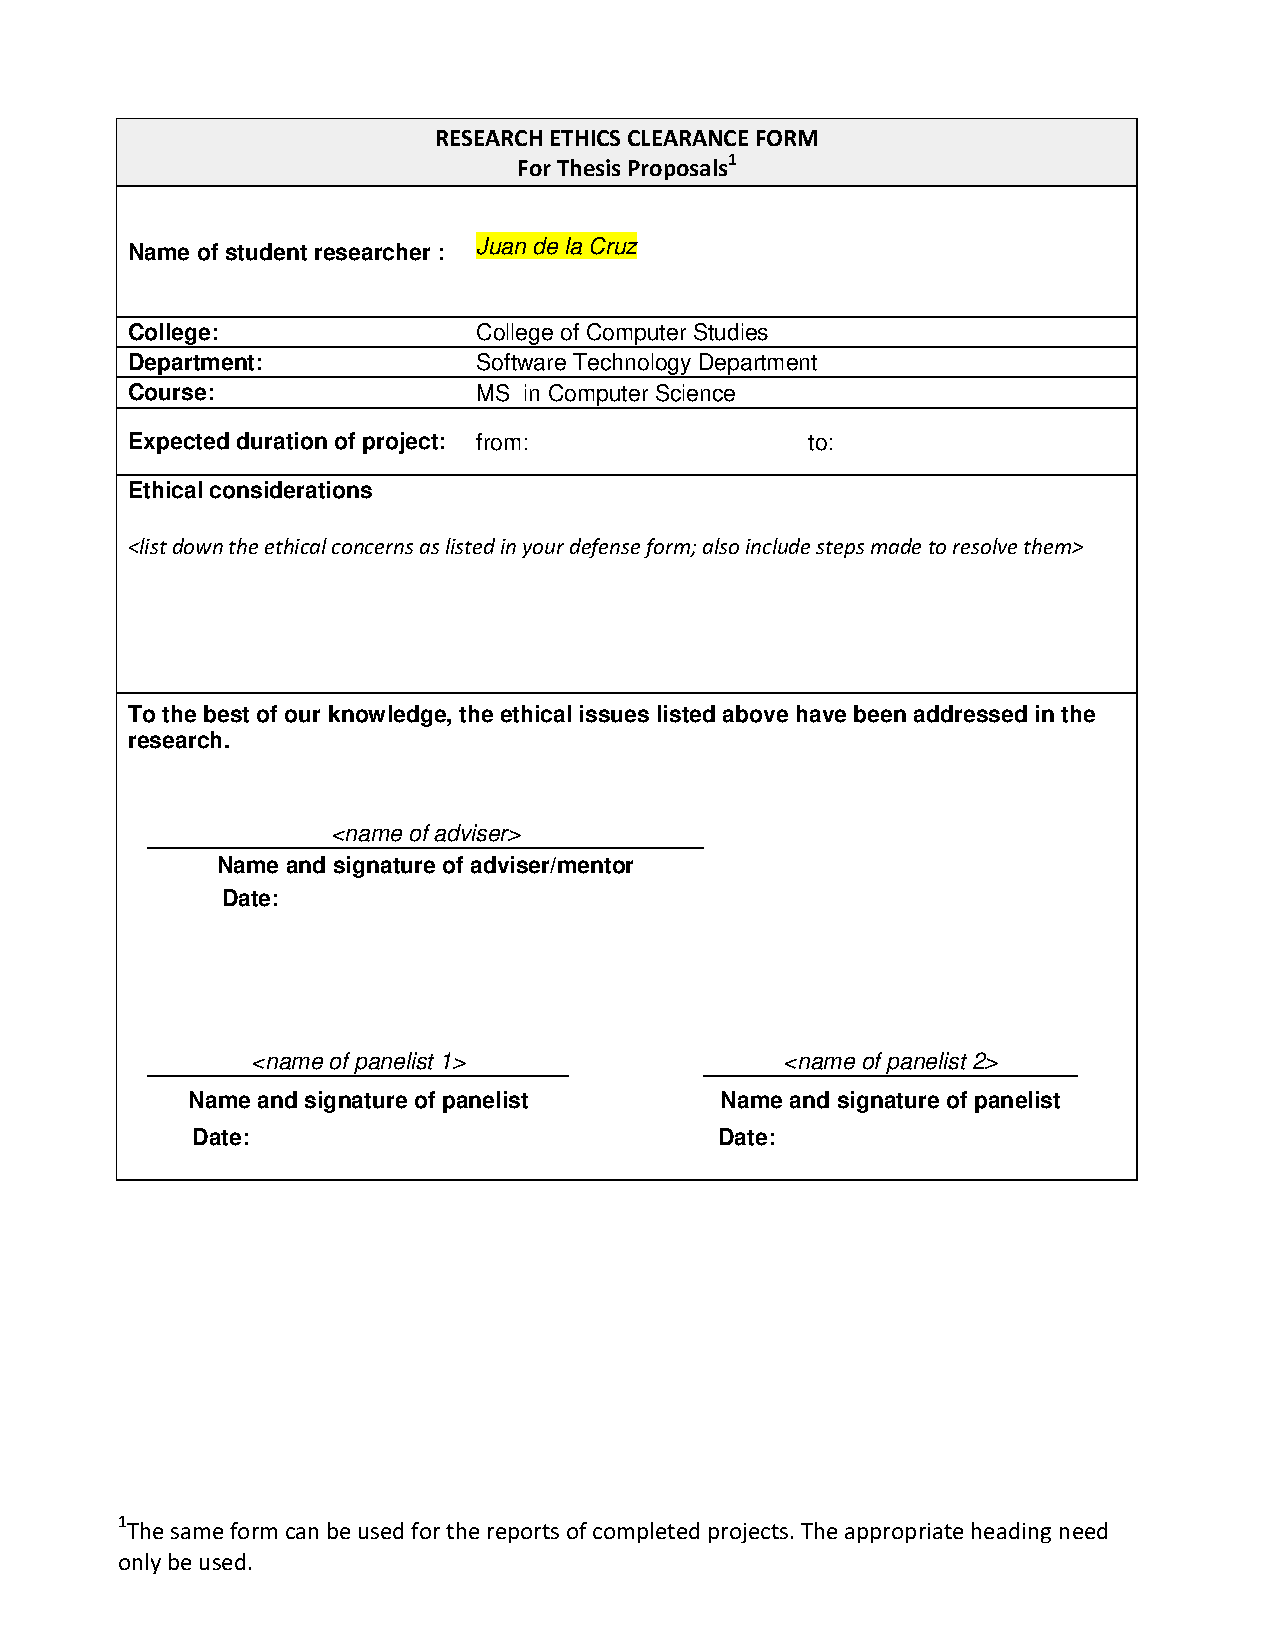
\includepdf[pages=-, scale = 0.9, pagecommand={}, offset = -30 0]{clearance.pdf}

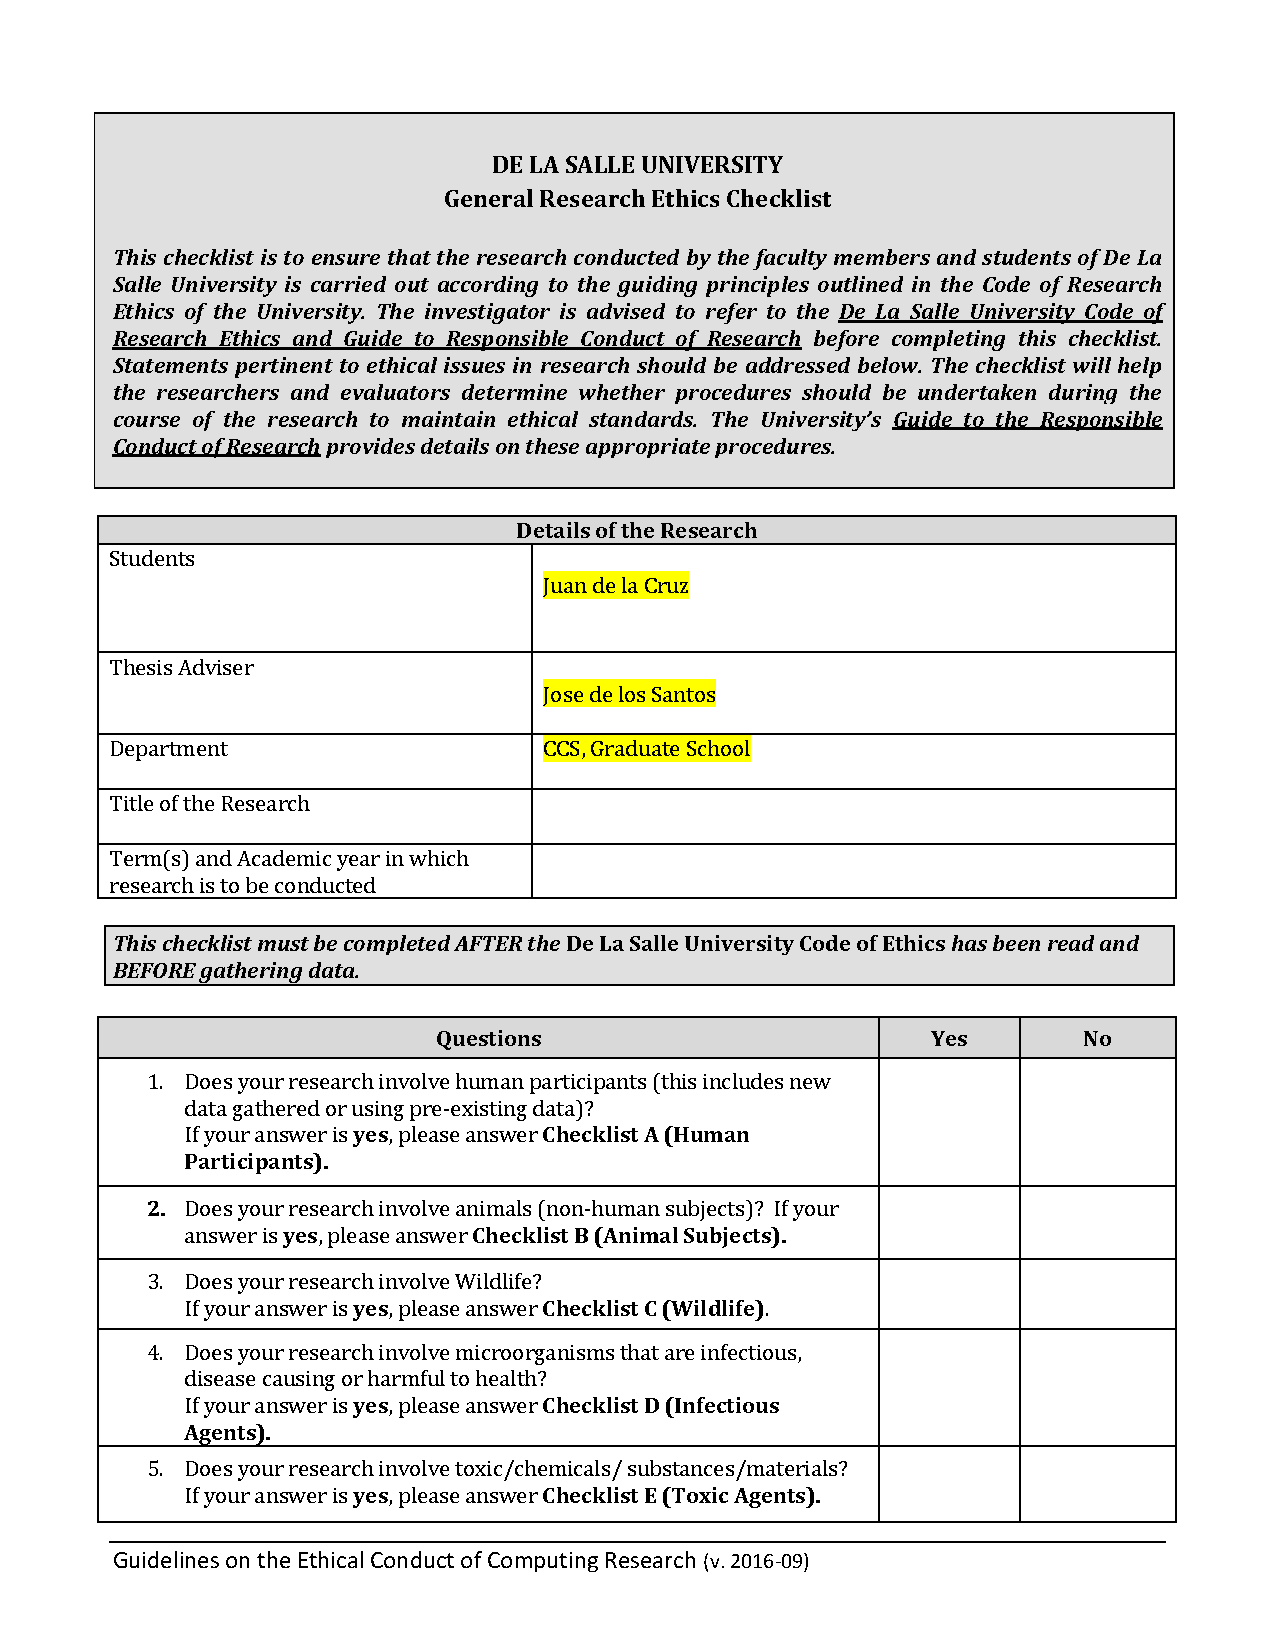
\includepdf[pages=-, scale = 0.9, pagecommand={}, offset = -30 0]{general_checklist.pdf}

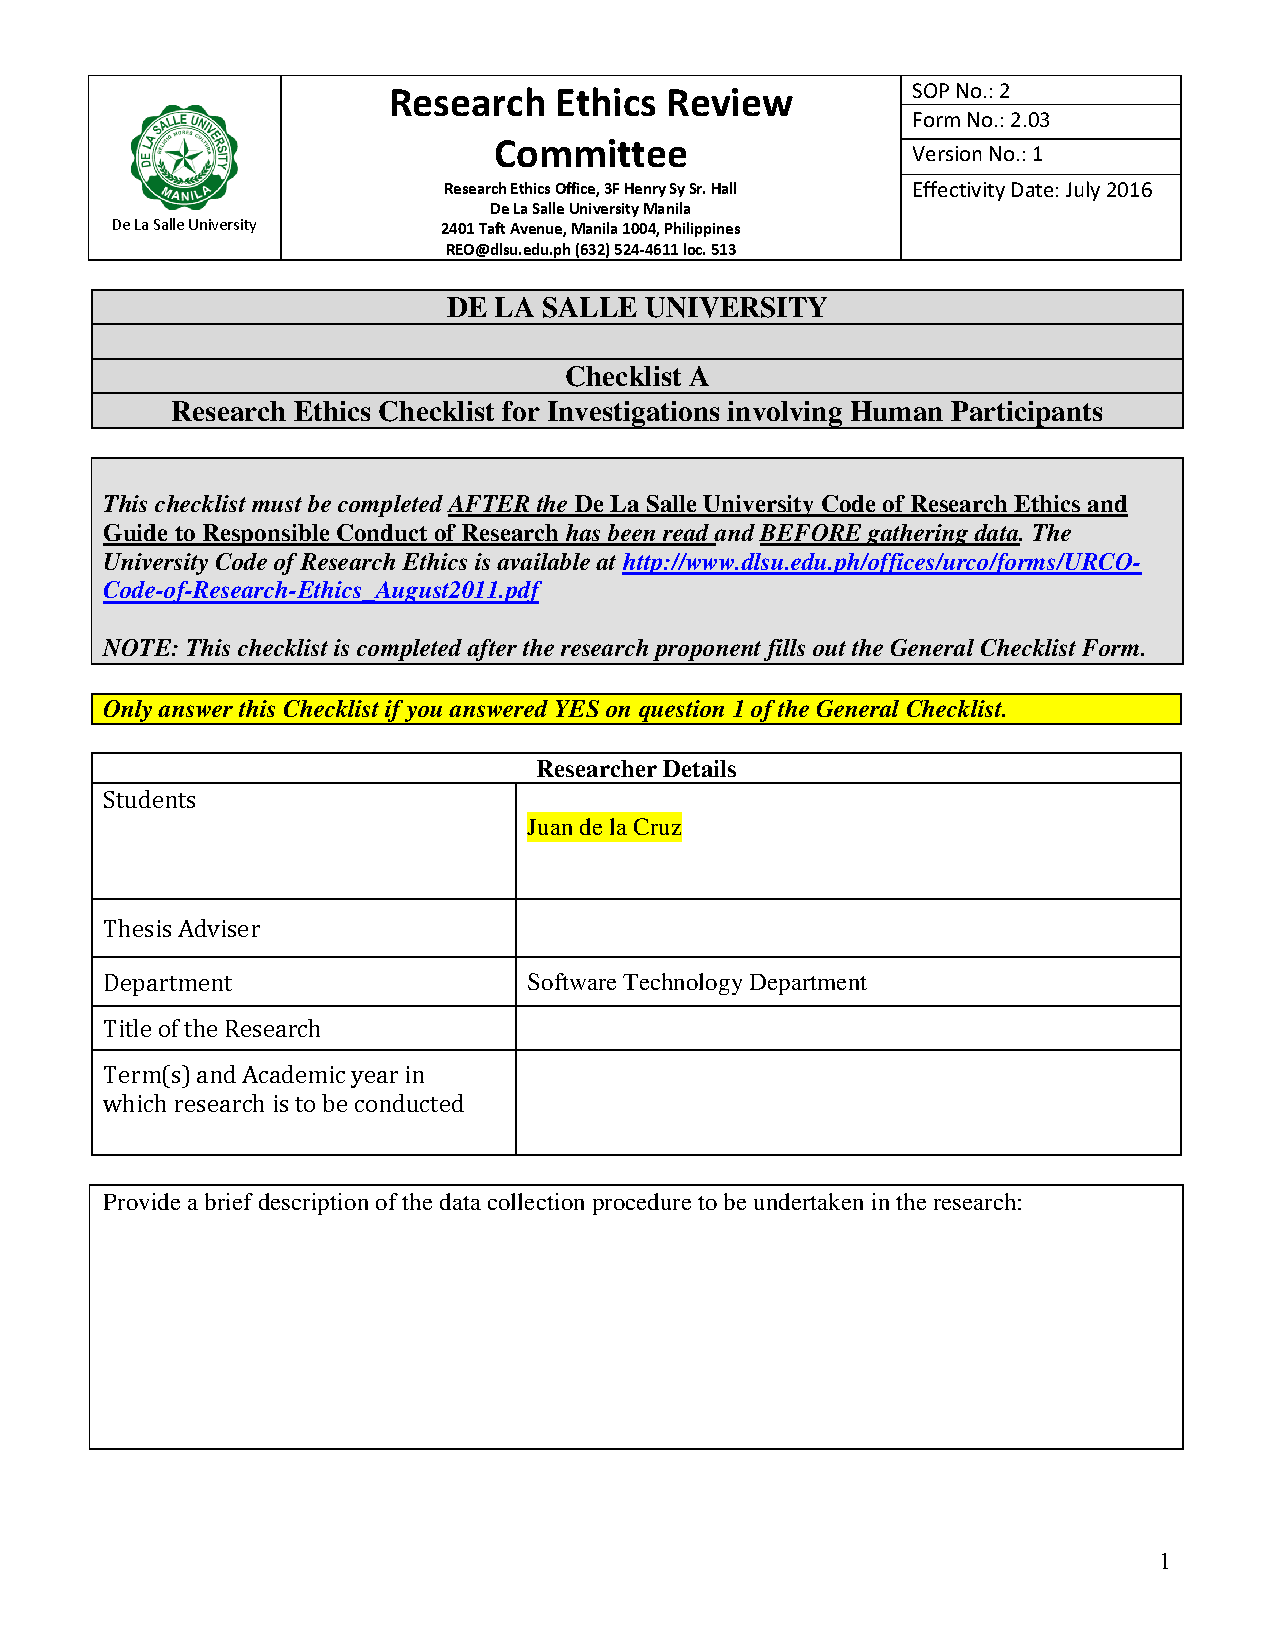
\includepdf[pages=-, scale = 0.9, pagecommand={}, offset = -30 0]{checklist-A.pdf}


              %-- includes LaTeX source file for Appendix A
                                  %-- your job: **CREATE/EDIT** your own source file for the appendices
% %%%%%%%%%%%%%%%%%%%%%%%%%%%%%%%%%%%%%%%%%%%%%%%%%%%%%%%%%%%%%%%%%%%%%%%%%%%%%%%%%%%%%%%%%%%%%%%%%%%%%%
%
%   Filename    : appendix_B.tex
%
%   Description : This file will contain information about your Resource Persons
%                 
%%%%%%%%%%%%%%%%%%%%%%%%%%%%%%%%%%%%%%%%%%%%%%%%%%%%%%%%%%%%%%%%%%%%%%%%%%%%%%%%%%%%%%%%%%%%%%%%%%%%%%

\chapter{Resource Persons}
\label{sec:appendixc}

%
%  Indicate your resource persons here:
%
%	<full name and title, e.g., Dr. Juan de la Cruz>
%	<profession, e.g., faculty>
%	<department, e.g., College of Computer Studies>
%	<name of institution, e.g., De La Salle University>
%	<e-mail address>
%
%

%
%  the following shows 3 examples, replace entries with your own
%
\newcommand{\resperson}[4]{\textbf{#1} \\ #2 \\ #3 \\ \url{#4}\vspace{0.5em}\\}

\resperson{Dr. Firstname1 Lastname1}{Adviser}{College of Computer Studies\\De La Salle University-Manila}{emailaddr@dlsu.edu.ph}
\resperson{Mr. Firstname2 Lastname2}{Role2}{Affiliation2}{emailaddr2@domain.com}
\resperson{Ms. Firstname3 Lastname3}{Role3}{Affiliation3}{emailaddr3@domain.net}




%\bibliographystyle{apacite}       %-- specified APA style for bibliograpy
                                  %-- more details about APA style citation can be found in www.ctan.org/tex-archive/biblio/bibtex/contrib/apacite/

                                  %-- bibliographic entries are handled via bibtex; refer to www.bibtex.org for more details


\bibliography{myreferences}       %-- the file "myreferences.bib" is a sample bibliography (bib) from SIGGRAPH 
                                  %-- your job: **CREATE/EDIT** your own bibliography file  

\end{document}

